%%
%% If you intend to use figures of formats jpg, png or pdf and want the
%% output to be immediately a pdf file, compile with pdflatex.
%%
%% If you want to use eps or ps figures, your output will be a dvi
%% file that can be converted to ps and pdf formats. In this case you
%% should compile your document with latex.
%%
%%This template is compatible with both methods.
%%
\title{{\normalsize Optimization and Algorithms} \\
Financial portfolio optimization}
\author{
        Bernardo Gomes
        \and
        Kishan Rama
        \and
        Tom\'as Falcato \\ {\tt bernardo.n.gomes@ist.utl.pt} \and {\tt kishan.rama@ist.utl.pt} \and {\tt tomas.falcato.costa@ist.utl.pt} \\
        Instituto Superior T\'{e}cnico}
\date{\today}


\documentclass[a4paper]{IEEEtran}
\usepackage[utf8]{inputenc}
\usepackage{graphicx}
\usepackage{amsmath}
\usepackage{amsfonts}
\usepackage{listings}

\begin{document}
\maketitle

\begin{abstract}
 Para o problema de \textit{Financial portfolio optimization}, dado um conjunto de \textit{assets}, pretende-se obter uma forma de distribuir o dinheiro a investir por forma a maximizar o retorno. A cada \textit{asset}, existe um risco associado, sendo que o risco de cada um poderá, ou não, influenciar o risco dos restantes.
%----------------------------------------------------------------------------------------------------------------
%PERGUNTAR!!!!!!!!!!!!!!!!!!!!!!!!!!!!!!!!!!!
Se considerarmos todas as variáveis inerentes à otimização deste tipo de problemas, iremos obter funções não convexas, pelo que se considera uma aproximação facilmente computável através de otimização convexa e cujos resultados, obtidos a partir do \textit{software CVX}, são bastante próximos dos ótimos. 
%----------------------------------------------------------------------------------------------------------------
%segunda parte do projeto
Posteriormente, o problema foi reformulado por forma a obter uma solução sub-ótima mas com menor tempo de computação. 
%----------------------------------------------------------------------------------------------------------------
%principais resultados
%PERGUNTAR!!!!!!!!!!!!!!!!!!!!!!!!!!!!!!!!!!!!!!!!!!!!!
%----------------------------------------------------------------------------------------------------------------
\end{abstract}

\smallskip
\noindent \textbf{Keywords.} Portfolio Optimization \textbullet CVX \textbullet Barrier Method \textbullet Newton Method

\section{Introdução}
\label{sec:introduction}
Este artigo pretende obter uma solução para o problema de \textit{Portfolio Optimization}. Para tal, a nossa abordagem maximiza o retorno esperado e minimiza o risco de investimento tendo em conta a aversão ao risco colocada pela pessoa que investe.

Na vida real, o problema discutido neste artigo tem extrema importância na medida em que praticamente todas as pessoas fazem investimentos do seu dinheiro. A formulação terá em conta não só os casos em que a pessoa pretende rápidos retornos e pretende que estes sejam bastante elevados, independentemente de o risco a ele associado ser relativamente elevado, como também casos cujo objetivo seja obter um resultado de longo prazo em que a aversão ao risco é um fator preponderante face à quantia recebida.

%contributions!!!!!!!!!!!!
Por forma a resolver, e melhor compreender o problema, numa primeira abordagem foi utilizado o \textit{software CVX}. Posteriormente, implementa-se a mesma resolução do problema, mas com este reescrito por forma a utilizar o algoritmo \textit{Barrier Method}. 


O artigo está organizado da forma enunciada de seguida. No capítulo
~\ref{sec:problem-formulation}, é introduzida a função a otimizar e as respetivas variáveis,  capítulo~\ref{sec:cvx} descreve a abordagem para a utilização do \textit{software CVX}, sendo esta alterada para a utilização do \textit{Barrier Method}, descrito no capítulo~\ref{sec:barrier-method}. Os resultados obtidos nas duas fases são discutidos e comparados em~\ref{sec:numerical-results}. As conclusões são apresentadas posteriormente em ~\ref{sec:conclusion}.

\section{Formulação do Problema}
\label{sec:problem-formulation}

Para a obtenção dos resultados do problema descrito anteriormente, a função utilizada foi a seguinte:
\begin{equation}
  \label{eq:problem}
\begin{array}[t]{ll} \text{maximize} & \mu^\top \omega - \gamma \omega^\top \Sigma \omega \\
\text{subject to} & 1^\top \omega = 1 \\ &  \omega \in \mathbb{R}_+^n \end{array}
\end{equation}

Apresenta-se de seguida a descrição das variáveis da função de otimização:

\begin{itemize}
\item  $\omega$ $\rightarrow$ vetor de dimensão \textit{n}, onde cada posição \textit{i}, contém a fração do dinheiro a investir no \textit{asset i} para obter o máximo de lucro. Será esta a variável que se pretende a maximizar;

\item $\mu$ $\rightarrow$ vetor de dimensão \textit{n}, onde cada posição \textit{i}, contém o retorno esperado para o \textit{asset i};

\item $\Sigma$ $\rightarrow$ matriz das covariâncias, de dimensão \textit{n}$\times$\textit{n} dos retornos dos \textit{assets}. É através deste parâmetro que se representa a influência que cada \textit{asset} tem nos restantes e vice-versa. Por exemplo, é de esperar que tendo um valor muito elevado na entrada \textit{ij} desta matriz, no caso de haver uma quebra nos retornos do \textit{asset i}, o \textit{asset j} irá, também sofrer quebra nos retornos, ou um aumento dos mesmos, dependendo do valor dessa entrada. Um caso real desta formulação é a forte dependência entre as ações do petróleo e dos automóveis ou a relação de competição entre cadeias concorrentes;

\item $\mu^\top \omega \rightarrow$ representa o retorno expectável do portfólio;

\item $\gamma \rightarrow$ variável que controla o \textit{tradeoff} entre o retorno e o risco. Será este parâmetro que irá controlar se se pretende investir dando preferência a maximizar o retorno, ou dando preferência à minimização do risco;

\item $\gamma \omega^\top \Sigma \omega \rightarrow$ representa a variância do retorno do portfólio. É o parâmetro que mede o risco de investimento;
\end{itemize}

A \textit{constraint} $1^\top \omega = 1$ indica que a soma dos investimentos no portfólio não pode ultrapassar o capital inicial. Note-se que os investimentos são uma fração do capital inicial e não o seu valor absoluto. Ao forçar que $\omega \in \mathbb{R}_+^n$ indica que não podem existir investimentos negativos. 
%Falar com o professor
Na prática esta situação poderia existir, no caso de termos capital num dado \textit{asset} e a melhor solução ser retirar o capital deste para investir noutro mais lucrativo.

Ao analisar a função que queremos otimizar, verifica-se que é quadrática, ou seja, do tipo $x^\top Ax+b^\top x+c$.
Para o contexto em questão, tem-se que maximize $\mu^\top \omega - \gamma \omega^\top \Sigma \omega \equiv$ minimize $\gamma \omega^\top \Sigma \omega + (- \mu^\top) \omega \equiv$ minimize $\omega^\top \gamma \Sigma \omega + (- \mu^\top) \omega$.

Sendo a matriz das covariâncias semi-definida positiva e simétrica, verifica-se que a nossa função é realmente quadrática sendo $A = \gamma \Sigma$, $b = -\mu$ e $c=0$. Sendo a função quadrática, podemos também concluir, que é convexa. Desta forma, a otimização será feita de acordo com esta propriedade.

\section{CVX}
\label{sec:cvx}
Por forma a implementar a solução apresentada na equação 1, e sendo esta convexa, utilizou-se o \textit{software CVX}\cite{CVX}. De seguida apresenta-se a parte do código de \textit{Matlab} onde se utiliza o \textit{CVX}.

\lstinputlisting{cvx.m}

\section{Barrier Method}
\label{sec:barrier-method}



\section{Numerical results}
\label{sec:numerical-results}

How does it really work in practice? Provide simulated performance
metrics. If possible, compare with other well-known methods.

Explain your experiments' setup to make it easily understandable and
replicable by a reader from the field that does not know your problem.

Comment your results. It might help to show a plot, as to illustrate
your commentary, like Figure~\ref{fig:solution-l1}.


The commentary of the plots should not just repeat the graphically
obvious such as "the solution is different from the original signal",
but explain, for example, how this difference relates to quick changes
on the signal. Is the solution too slow to follow the signal
variations? What is the magnitude of the error?

\begin{figure}[htp]
  \centering
  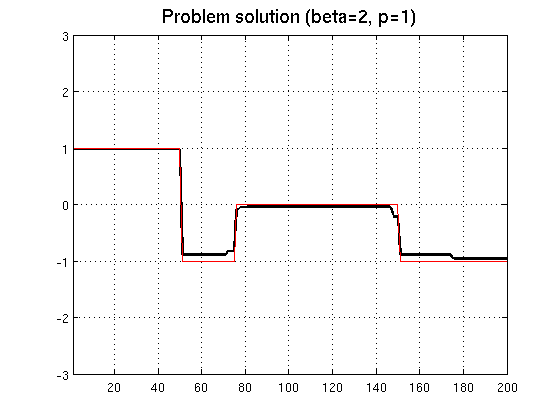
\includegraphics[width=0.9\columnwidth]{./solution1}
  \caption{Solution for the L1 norm cost function.}
  \label{fig:solution-l1}
\end{figure}

You might also want to vary the problem's parameters and see how the
solution evolves. Don't forget to explain why is the choice of
parameters in the solution depicted in Figure~\ref{fig:solution-l1}
better than the others.

Figures should be chosen wisely. You can never lay out the whole
parameter space, so provide insight into which parameters are
significant over what range and which ones are less important.



\section{Conclusions}
\label{sec:conclusion}

In general a short summarizing paragraph will be sufficient. It should
not simply repeat material from the Abstract or Introduction. In some
cases it's possible to now make the original claims more concrete,
\textit{e.g.}, by referring to quantitative results.


\begin{thebibliography}{9}

\bibitem{CVX}
  [CVX15] \texttt{http://cvxr.com/cvx}, Junho 2015

\end{thebibliography}

\end{document}
This is never printed 